\documentclass[a4paper,12pt]{extarticle}
\usepackage{geometry}
\usepackage[T1]{fontenc}
\usepackage[utf8]{inputenc}
\usepackage[english,russian]{babel}
\usepackage{amsmath}
\usepackage{amsthm}
\usepackage{amssymb}
\usepackage{fancyhdr}
\usepackage{setspace}
\usepackage{graphicx}
\usepackage{colortbl}
\usepackage{tikz}
\usepackage{pgf}
\usepackage{subcaption}
\usepackage{listings}
\usepackage{indentfirst}
\usepackage[
backend=biber,
style=numeric,
maxbibnames=99
]{biblatex}
\addbibresource{refs.bib}
\usepackage[colorlinks,citecolor=blue,linkcolor=blue,bookmarks=false,hypertexnames=true, urlcolor=blue]{hyperref} 
\usepackage{indentfirst}
\usepackage{mathtools}
\usepackage{booktabs}
\usepackage[flushleft]{threeparttable}
\usepackage{tablefootnote}

\usepackage{chngcntr} % нумерация графиков и таблиц по секциям
\counterwithin{table}{section}
\counterwithin{figure}{section}

\graphicspath{{graphics/}}%путь к рисункам

\makeatletter
% \renewcommand{\@biblabel}[1]{#1.} % Заменяем библиографию с квадратных скобок на точку:
\makeatother

\geometry{left=2.5cm}% левое поле
\geometry{right=1.0cm}% правое поле
\geometry{top=2.0cm}% верхнее поле
\geometry{bottom=2.0cm}% нижнее поле
\setlength{\parindent}{1.25cm}
\renewcommand{\baselinestretch}{1.5} % междустрочный интервал


\newcommand{\bibref}[3]{\hyperlink{#1}{#2 (#3)}} % biblabel, authors, year
\addto\captionsrussian{\def\refname{Список литературы (или источников)}} 

\renewcommand{\theenumi}{\arabic{enumi}}% Меняем везде перечисления на цифра.цифра
\renewcommand{\labelenumi}{\arabic{enumi}}% Меняем везде перечисления на цифра.цифра
\renewcommand{\theenumii}{.\arabic{enumii}}% Меняем везде перечисления на цифра.цифра
\renewcommand{\labelenumii}{\arabic{enumi}.\arabic{enumii}.}% Меняем везде перечисления на цифра.цифра
\renewcommand{\theenumiii}{.\arabic{enumiii}}% Меняем везде перечисления на цифра.цифра
\renewcommand{\labelenumiii}{\arabic{enumi}.\arabic{enumii}.\arabic{enumiii}.}% Меняем везде перечисления на цифра.цифра

\begin{document}
\begin{titlepage}
\newpage

{\setstretch{1.0}
\begin{center}
ПРАВИТЕЛЬСТВО РОССИЙСКОЙ ФЕДЕРАЦИИ\\
ФГАОУ ВО НАЦИОНАЛЬНЫЙ ИССЛЕДОВАТЕЛЬСКИЙ УНИВЕРСИТЕТ\\
«ВЫСШАЯ ШКОЛА ЭКОНОМИКИ»
\\
\bigskip
Факультет компьютерных наук\\
Образовательная программа «Прикладная математика и информатика»
\end{center}
}

\vspace{7em}

\begin{center}
{\bf ВЫПУСКНАЯ КВАЛИФИКАЦИОННАЯ РАБОТА}\\
%Выберите какой у вас проект
{\bf Исследовательский проект на тему:}\\
%{\bf Программный проект на тему:}\\
%{\bf Отчет о командном программном проекте на тему:}\\
{\bf Сжатие словарей для нейросетевого анализа исходных кодов программ}\\
\end{center}

\vspace{2em}

{\bf Выполнил студент: \vspace{2mm}}

{\setstretch{1.1}
\begin{tabular}{l@{\hskip 1.5cm}l}
группы \#БПМИ171, 4 курса & Гусев Андрей Алексеевич 
\end{tabular}}

% Обычно у вас есть один научный руководитель, и это человек, с которым вы работаете над проектом. Иногда по формальным причинам у вас будет руководитель (штатный сотрудник Вышки) и соруководитель (тот, с кем вы работаете), — об этом вам сообщит учебный офис (в случае с ВКР) или ЦППРиП (в случае с курсовым проектом). Также, если кто-то дополнительно вам помогал, то его можно указать как консультанта. 

%ваш официальный научник (из ВШЭ)
\vspace{1em}
{\bf Принял руководитель ВКР: \vspace{2mm}}

{\setstretch{1.1}
\begin{tabular}{l}
Чиркова Надежда Александровна\\
Научный сотрудник\\
Факультет компьютерных наук НИУ ВШЭ 
\end{tabular}}

% со-руководитель (если есть)
%\vspace{1em}
%{\bf Соруководитель: \vspace{2mm}}%это ваш официальный научник

%{\setstretch{1.1}
%\begin{tabular}{l}
%Петрова Надежда Александровна\\
%Инженер-исследователь\\
%ОАО Компания "Нейросети и деревья" 
%\end{tabular}}

% консультант (если есть)
%\vspace{1em}
%{\bf Консультант: \vspace{2mm}}%это ваш официальный научник

%{\setstretch{1.1}
%\begin{tabular}{l}
%Иванова Надежда Александровна\\
%Инженер-исследователь\\
%ОАО Компания "Нейросети и деревья" 
%\end{tabular}}

\vspace{\fill}

\begin{center}
Москва 2024
\end{center}

\end{titlepage}% это титульный лист - выберите подходящий вам из имеющихся в проекте вариантов (kr - курсовая работа у 3 курса, vkr - выпускная квалификационная работа у 4 курса)
\newpage
\setcounter{page}{2}

{
	\hypersetup{linkcolor=black}
	\tableofcontents
}

\newpage

\newpage
\section*{Аннотация}   % this is how to use russian
Ваша аннотация на русском языке.

\addcontentsline{toc}{section}{Аннотация}

\section*{Ключевые слова}
Глубинное обучение, разреживание моделей, рекуррентные нейронные сети
\pagebreak

\newpage
\section*{Введение}   % this is how to use russian
В современном мире маркетплейсы стали неотъемлемой частью электронной коммерции, предоставляя платформы для продажи товаров и услуг различным производителям и ритейлерам.
В 2023 году маркетплейсы продолжили быть главной движущей силой российской онлайн-торговли. Рост объема трат на маркетплейсах в 1,5 раза по сравнению с предыдущим годом свидетельствует о том, что интерес потребителей к онлайн-покупкам только укрепляется. На это влияют общерыночные факторы: продолжают развиваться альтернативные каналы поставок продукции ушедших брендов, улучшаются условия доставки, повышается удобство пользования платформами, расширяется сеть пунктов выдачи.

Согласно исследованиям Tinkoff Ecommerce, количество транзакций на маркетплейсах за год выросло на 63\% (см. рисунок ~\ref{fig:marketplaces-purchases-increased}). Лидерами по росту количества покупок стали Мегамаркет (число транзакций выросло в 4,3 раза), Wildberries (в 2 раза) и Ozon (в 1,6 раза).

\begin{figure}[hbtp]
	\centering
	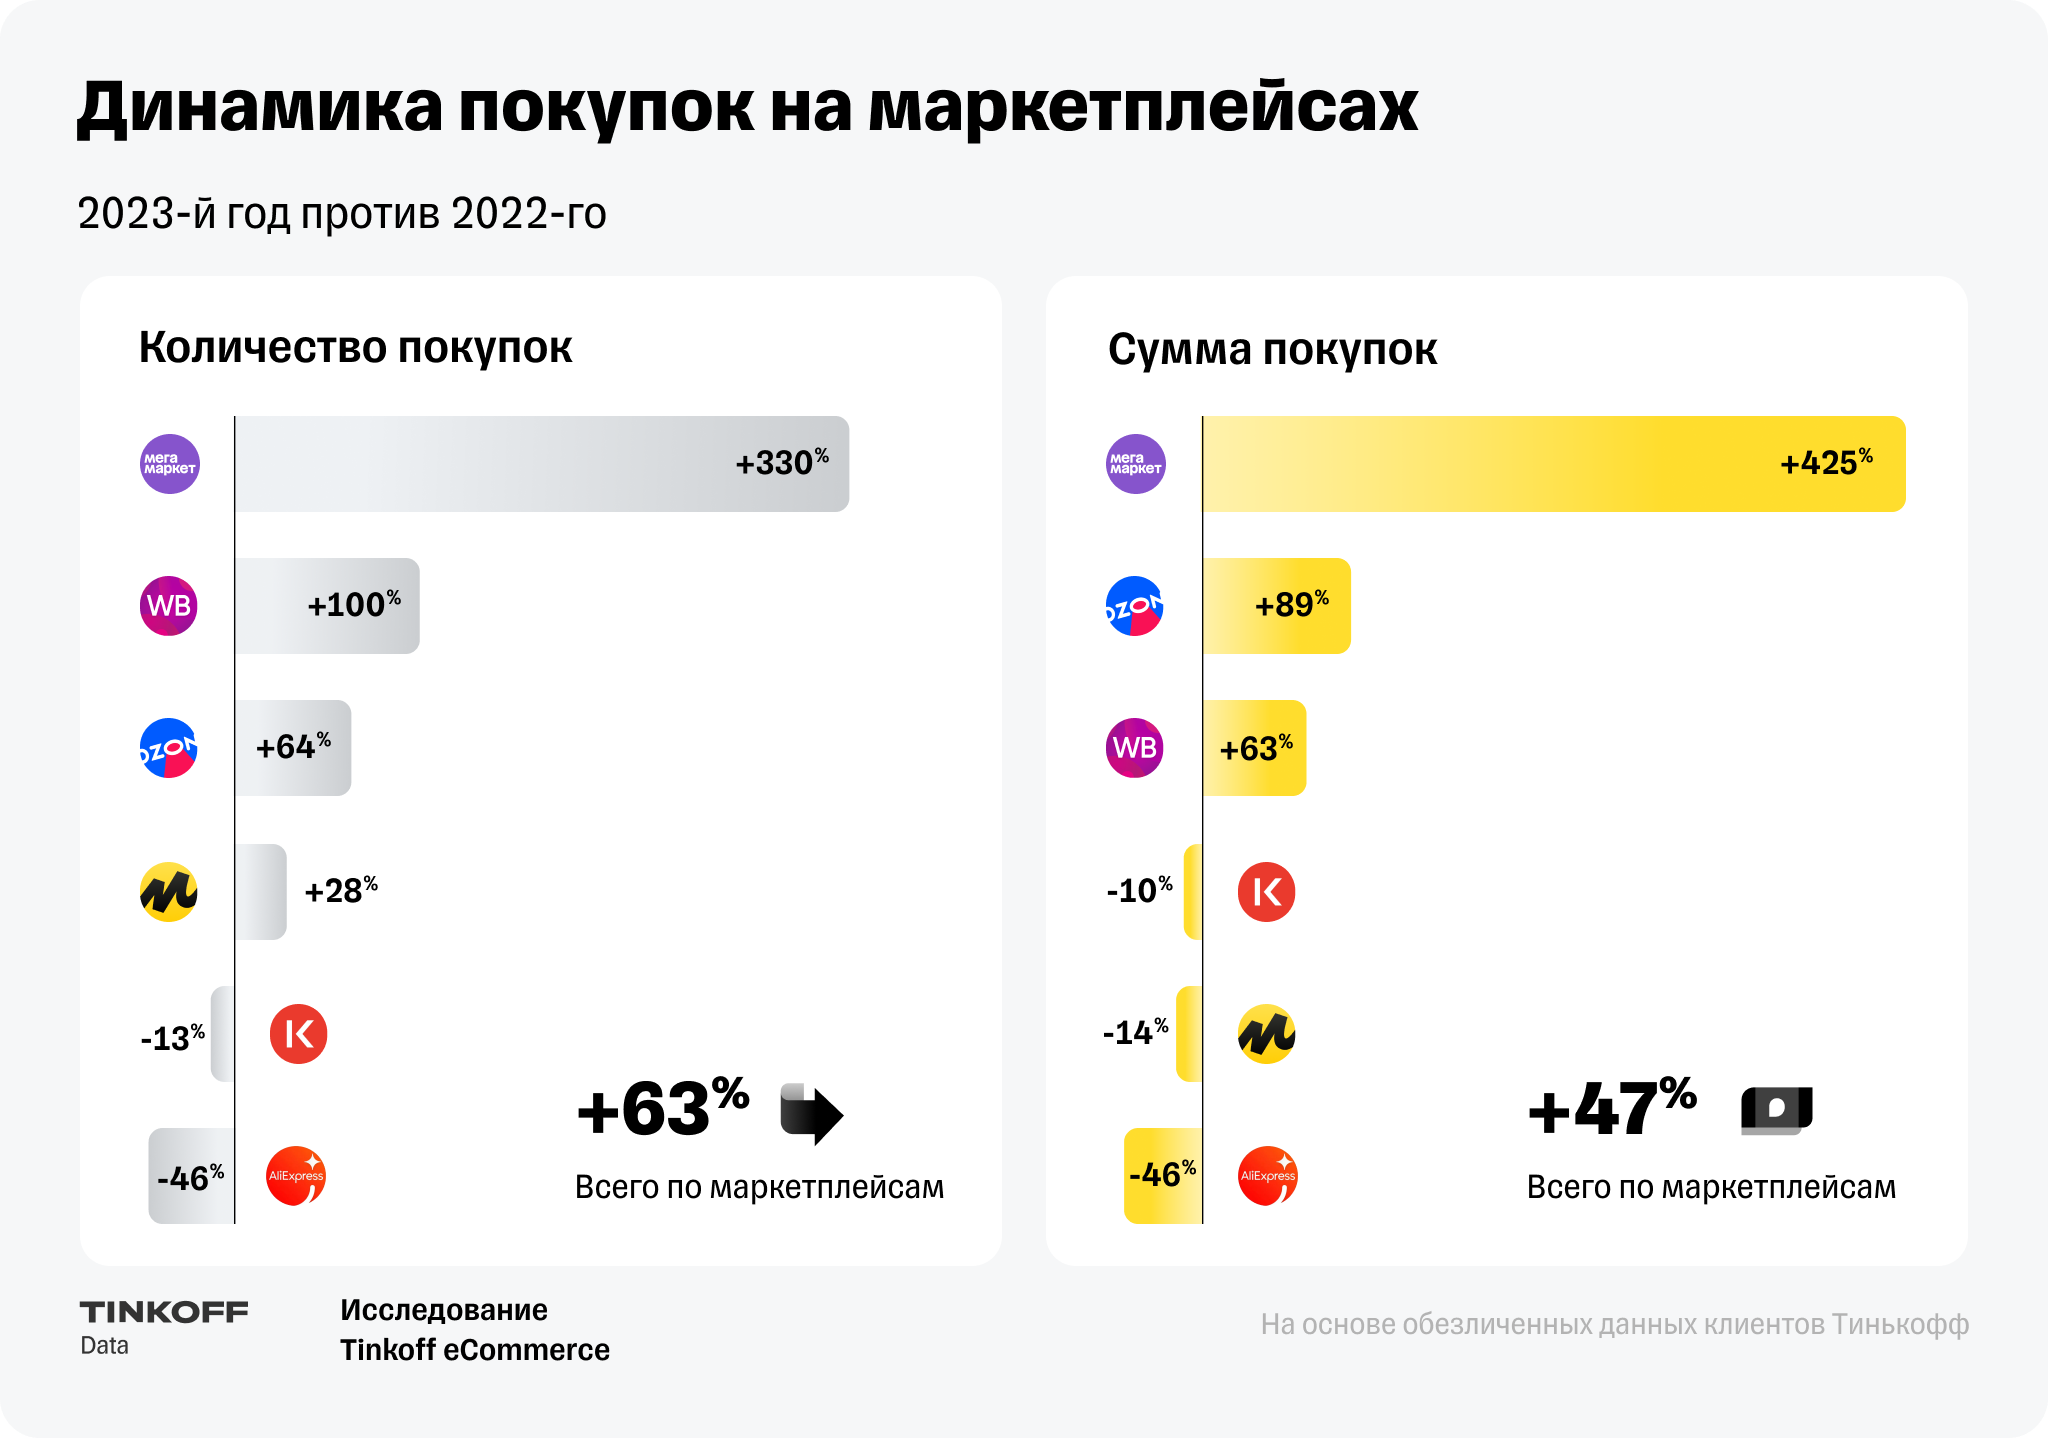
\includegraphics[scale=0.3]{marketplaces-purchases-increased.png}
	\caption{Динамика покупок на маркетплейсах в регионах.}
	\label{fig:marketplaces-purchases-increased}
\end{figure} 

Появился тренд на рост популярности маркетплейсов в российских регионах. В 2023 году жители российских городов стали значительно активнее совершать покупки на маркетплейсах: выросло как количество транзакций на онлайн-площадках, так и их сумма (см. рисунок ~\ref{fig:marketplaces-regions}). По количеству совершенных транзакций особенно заметен рост в таких городах, как Омск (+91\%), Красноярск (+88\%), Новосибирск (+79\%), Челябинск (+79\%) и Волгоград (+75\%). В Москве зафиксирован наименьший прирост числа транзакций (+41\%). Увеличение интереса жителей регионов к маркетплейсам объясняется рядом причин: расширением географии присутствия площадок, развитием сетей ПВЗ и логистических сервисов, улучшением условий доставки.

\begin{figure}[hbtp]
	\centering
	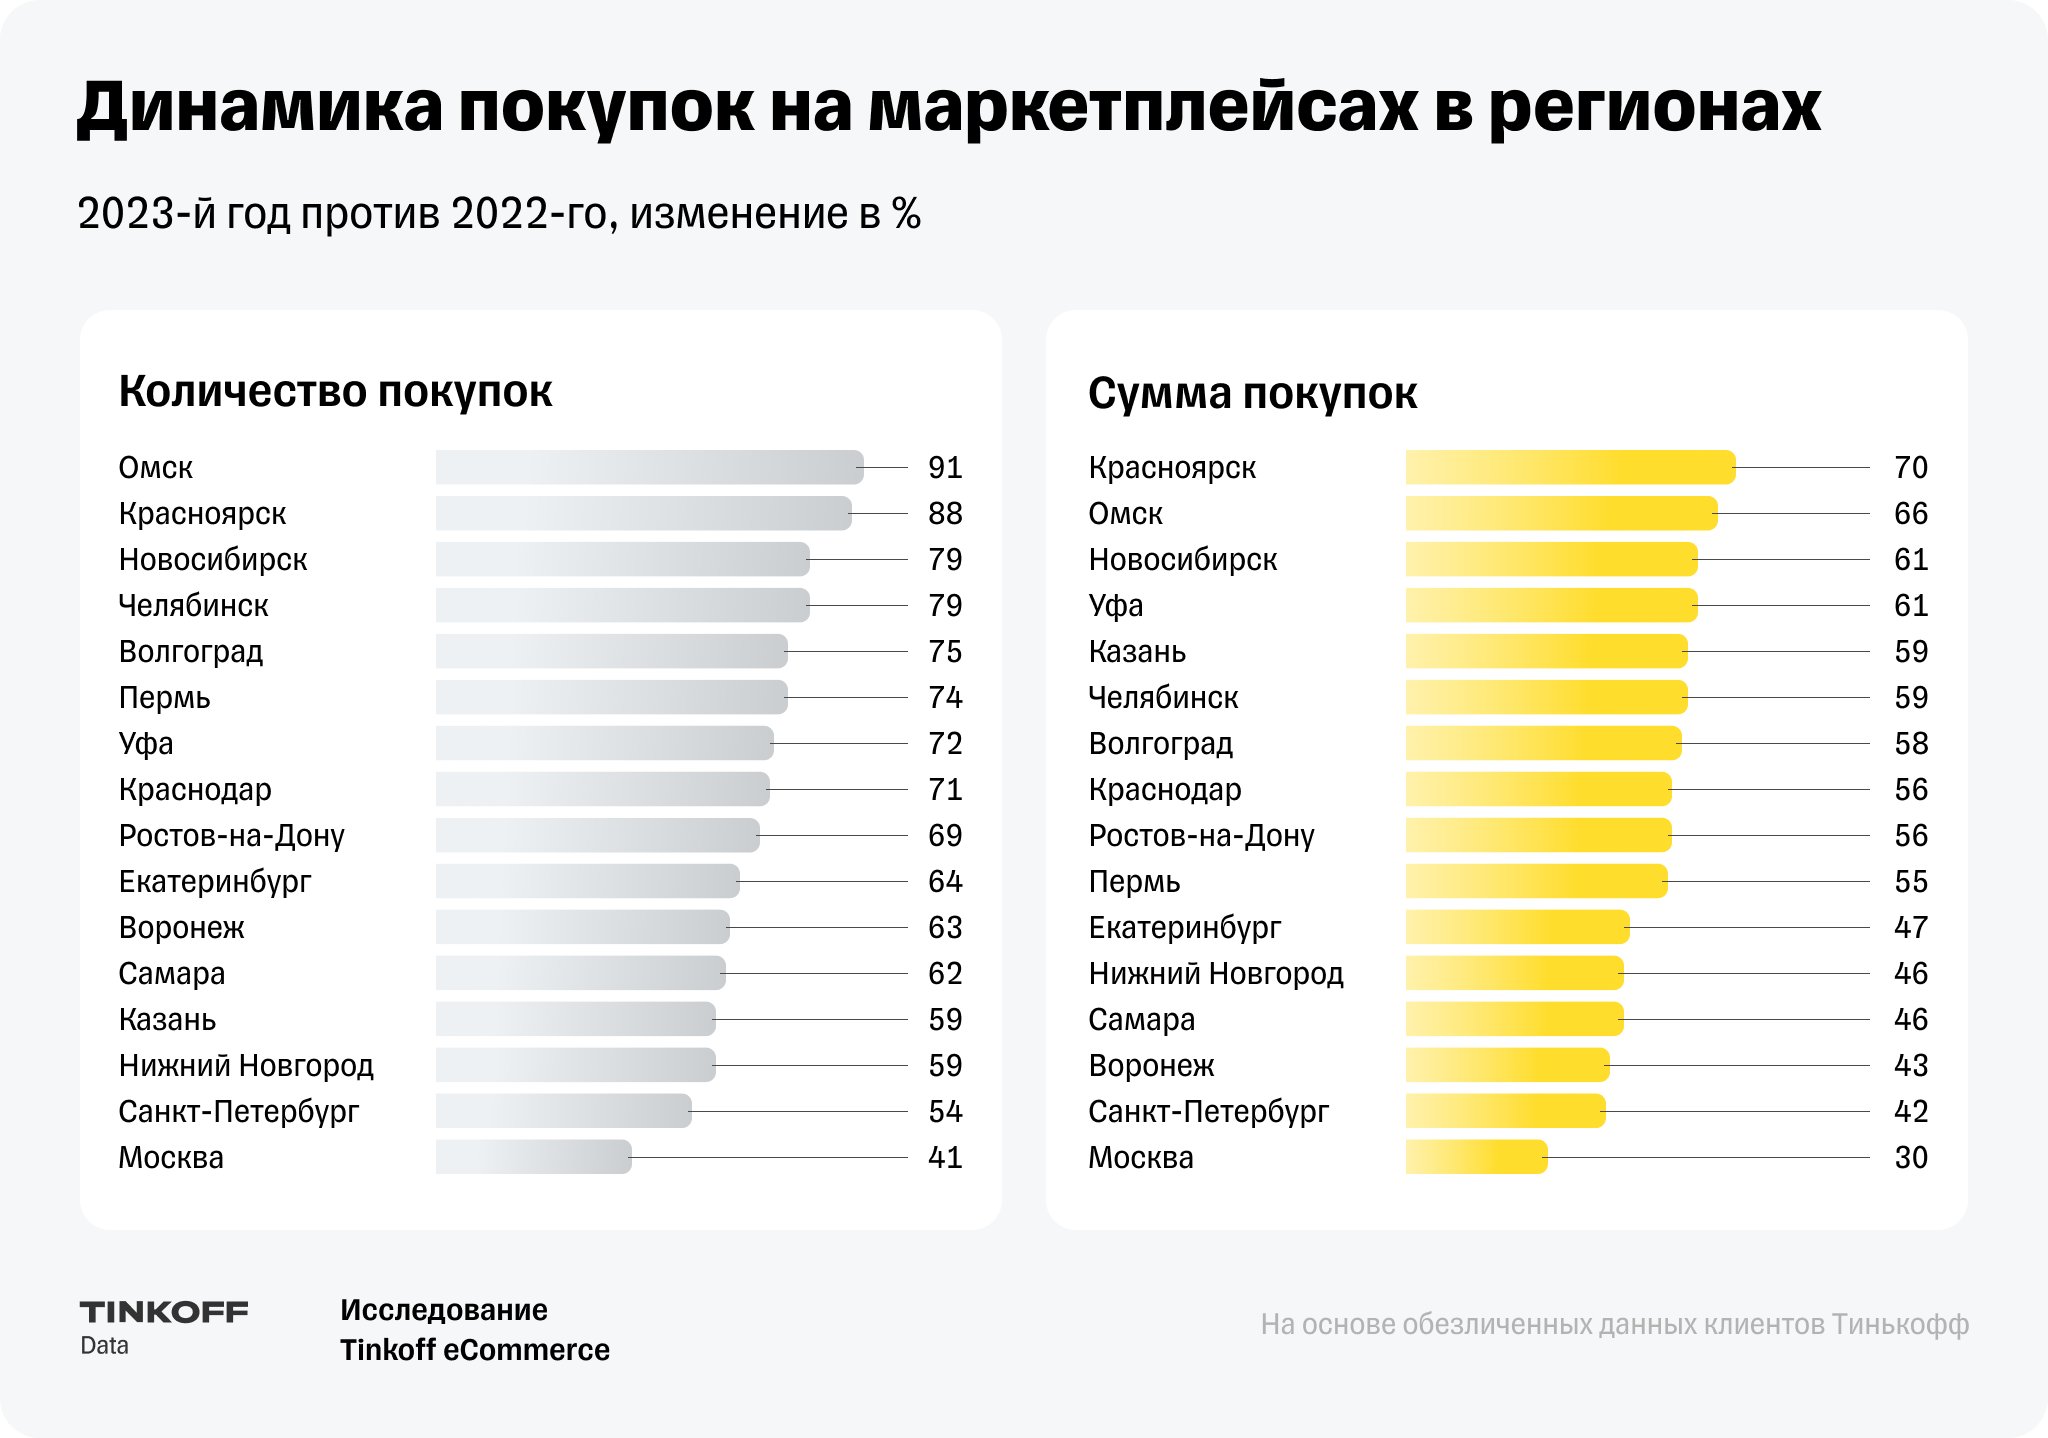
\includegraphics[scale=0.3]{marketplaces-regions.png}
	\caption{Динамика покупок на маркетплейсах в регионах.}
	\label{fig:marketplaces-regions}
\end{figure}  

Вместе с тем выросло количество селлеров на 8\%. Рынок становится более зрелым: место неопытных продавцов занимают более профессиональные. Они ведут бизнес более уверенно, укрепляют свои позиции на площадках и торгуют на нескольких платформах одновременно. Количество селлеров, ведущих торговлю на двух и более маркетплейсах, за год увеличилось на 17\%. Самой привлекательной платформой для старта бизнеса является Wildberries: 63\% продавцов в конце 2023 года выбирали ее в качестве первой площадки (см. рисунок ~\ref{fig:marketplaces-top}).

\begin{figure}[hbtp]
	\centering
	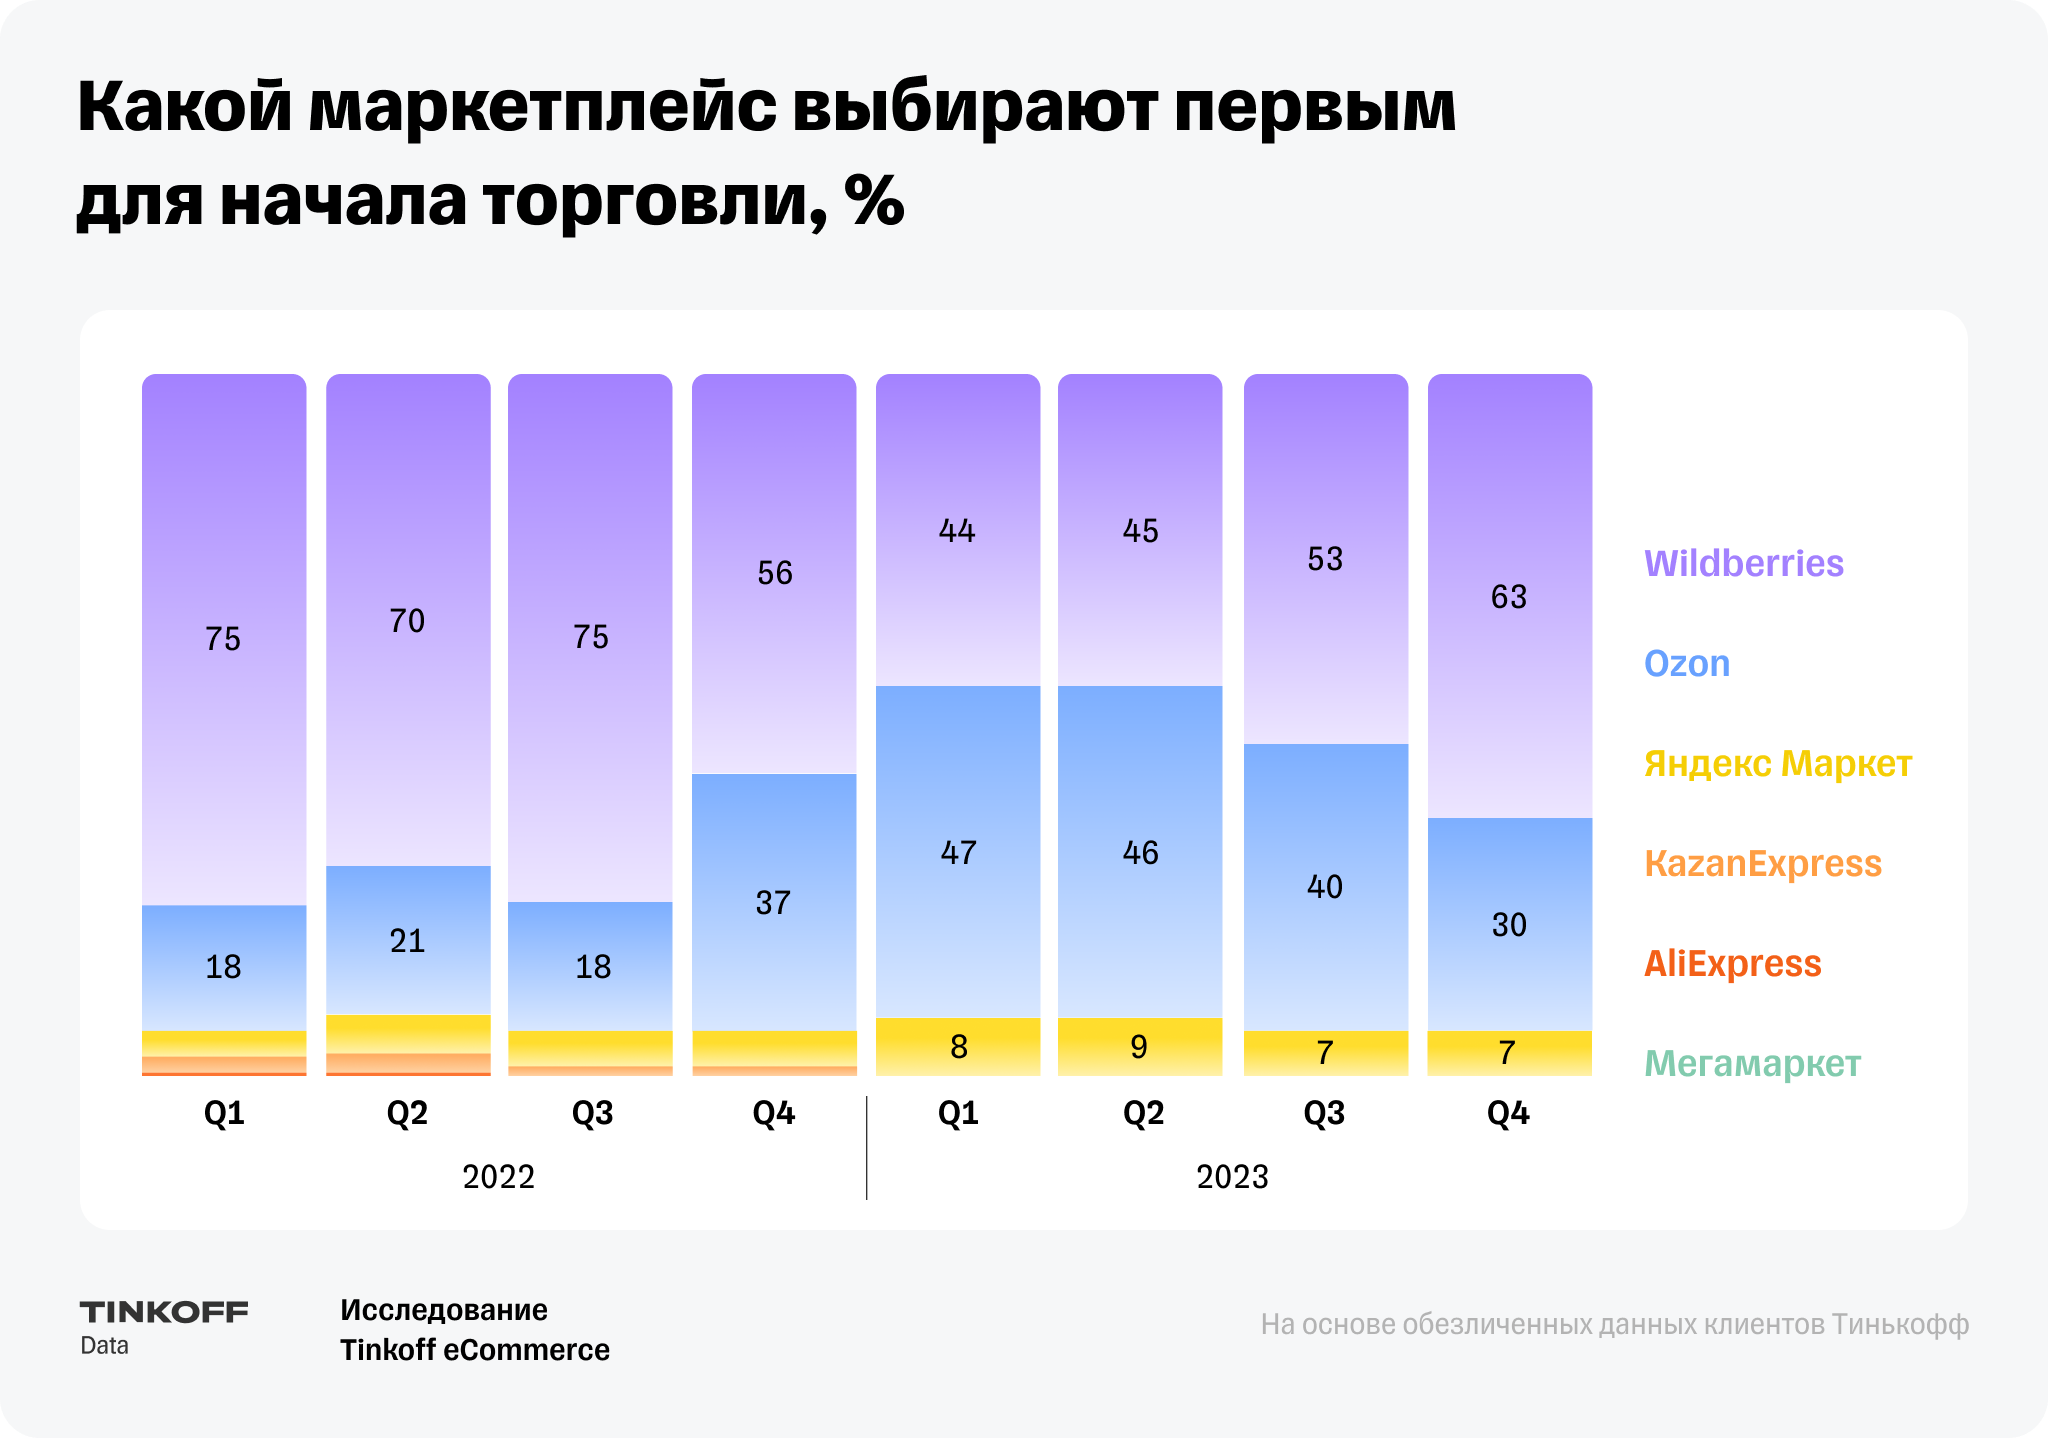
\includegraphics[scale=0.3]{marketplaces-top.png}
	\caption{Популярность маркетплейсов за 2023 год.}
	\label{fig:marketplaces-top}
\end{figure} 

С увеличением конкуренции продавцы все чаще обращаются к системам, которые могут помочь им в продажах, а также автоматизировать процесс работы. Одним из ключевых факторов успешной продажи становится эффективная SEO-оптимизация карточек товаров. Подбор наиболее подходящей категории и создание продаваемого описания, содержащего ключевые слова, позволяет улучшить видимость товаров в результатах поиска как на самом маркетплейсе, так и в поисковых системах, что напрямую влияет на увеличение продаж.

На данный момент существуют несколько сервисов (например, TurboTextPro, CopyMonkey, Gerwin), позволяющих сгенерировать описание товаров по характеристикам, ключевым словам или фото. Однако, качество сгенерированных описаний не всегда позволяют использовать их в системах автономного управления. В настоящее время российский рынок не предлагает специальных технологий и решений для подбора наиболее подходящей категории товара на маркетплейсе. Таким образом, задача создания качественного инструмента для эффективной SEO-оптимизации карточек товаров является актуальной. 

Цель данной работы — разработать сервис, в основе которого будет реализован функционал, способный классифицировать товары на маркетплейсе на основе их фотографий и генерировать соответствующие к ним описания. Сервис реализуется для маркетплейса Wildberries, так как он представляют наибольшую популярность у продавцов и покупателей. В качестве дальнейшего развития проекта можно рассмотреть другие площадки.

Для достижения поставленной цели необходимо решить следующие задачи:
\begin{itemize}
	\item подготовить набор данных, содержащий изображения товаров и соответствующие им категории и текстовые описания;
	\item провести исследование текущих архитектур нейронных сетей, используемых для классификации изображений и генерации текста, и на основе этого исследования выбрать наиболее подходящую архитектуру или их комбинацию для решения поставленной задачи;
	\item обучить выбранную нейронную сеть на подготовленных данных, оптимизировать и настроить параметры модели для повышения её производительности и качества результатов, а затем оценить эффективность реализованной архитектуры нейронной сети;
	\item интегрировать модель в программное обеспечение.
\end{itemize}


\section{Примеры} 
\subsection{Ссылки на статьи}

Ссылки на статьи оформляются с помощью пакета \texttt{biblatex}, например~\cite{chirkova18}. В описании статье в bib файле нужно обязательно указывать место публикации работы (журнал или конференцию) и год. Обратите внимание, что для описания статей из разных источников в списке литературы используются разные команды в bib файле: статья из журнала~\cite{ctan}, статья с конференции~\cite{chirkova18}, книга~\cite{knuth-acp}, глава книги~\cite{knuth-fa}. Если статься еще не опубликована нигде, а только выложена на arXiv, то на нее тоже можно сослаться~\cite{chirkova18_arxiv}, но предпочтительно ссылаться на опубликованную версию, если она уже существует. Если вы хотите сослаться на сайт, то можно либо так же внести его в список литературы~\cite{knuthwebsite} (рекомендуется, если таких ссылок у вас много из-за особенностей темы вашего проекта), либо использовать ссылку внизу страницы\footnote{Книги доступны по ссылке: \url{http://www-cs-faculty.stanford.edu/~uno/abcde.html}, дата обр. 16.05.2013}. При работе с онлайн ресурсами не забывайте указывать дату обращения к этому ресурсу, так как в отличие от опубликованных статей, эти ресурсы могут измениться в любой момент.

\subsection{Рисунки}

\begin{figure}[ht]
	\centering
	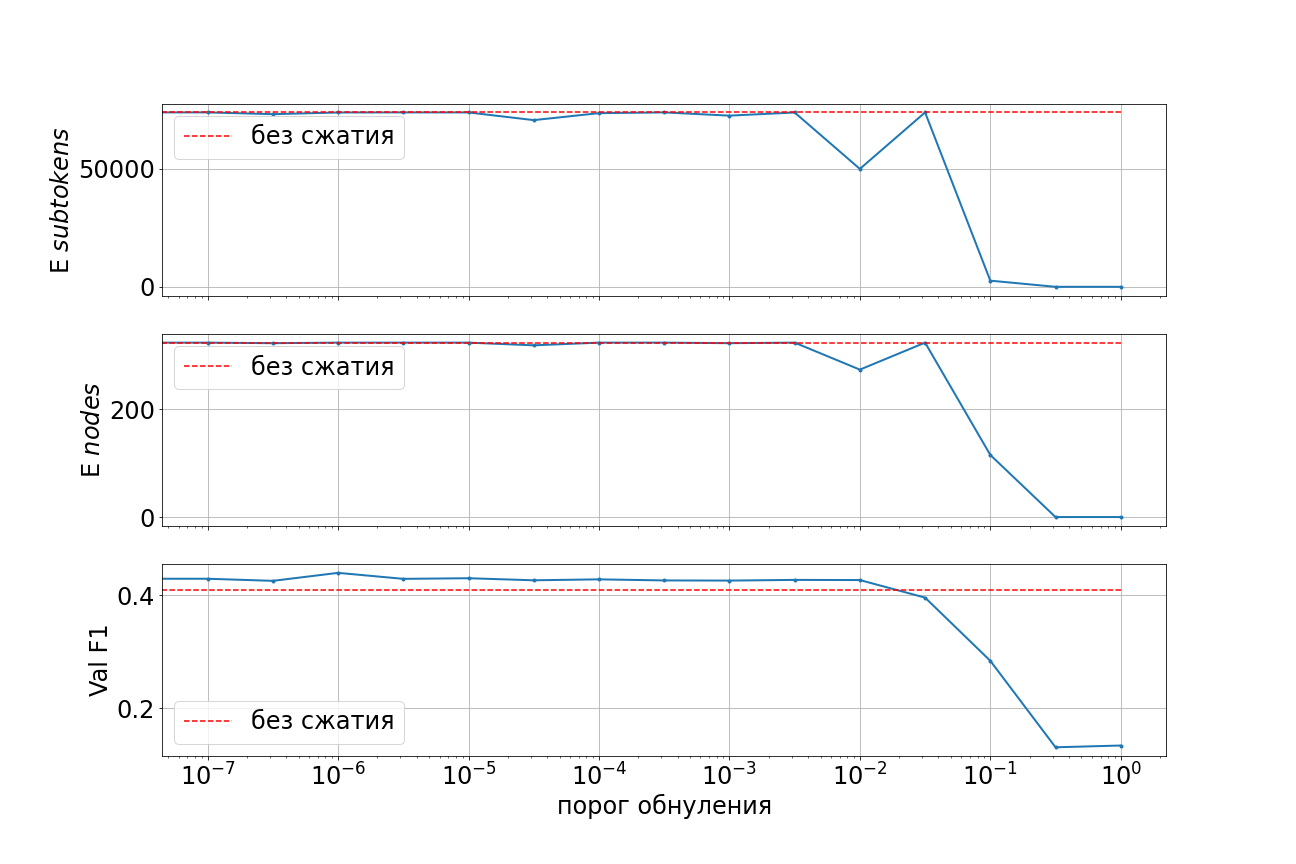
\includegraphics[width=0.8\textwidth]{example.png}
	\caption{Пример графика. Тут должна быть подпись, поясняющая что происходит на рисунке (краткая, но достаточная для понимания основной идеи графика).}
	\label{fig:by_epochs}
\end{figure}

Все рисунки в тексте должны иметь подписи и вы на них должны ссылаться в тексте. Например, на Рисунке~\ref{fig:by_epochs} изображен пример графика. Не забывайте подписывать все оси на графиках, добавлять легенду и пояснять все обозначения, а также используйте адекватного размера шрифты и толщину линий на графиках (все должно быть видно и понятно без многократного увеличения). На рисунке из примера явно не хватает обозначения синей линии в легенде.


\subsection{Таблицы}

Все таблицы в тексте тоже должны иметь подписи и вы на них должны ссылаться в тексте. Например, в Таблице~\ref{table:long_epochs} показаны результаты примерного эксперимента. 


\begin{table}[ht]
	\caption{Пример таблички. Тут должна быть подпись, поясняющая что происходит в таблице (краткая, но по делу).}
	\label{table:long_epochs}
	\footnotesize
	\centering
	\begin{tabular}{lrrrrrrrr}
		\toprule
		& \multicolumn{3}{c}{$\mathsf{Val}$} &
		\multicolumn{3}{c}{$\mathsf{Test}$} \\
		\cmidrule(lr){2-4} \cmidrule(l){5-7} 
		{} &  $\mathsf{Prec}$ &  $\mathsf{Rec}$ &  $\mathsf{F1}$ &  $\mathsf{Prec}$ &  $\mathsf{Rec}$ &  $\mathsf{F1}$  &  $\mathsf{nodes}$ & $\mathsf{subtokens}$\\
		\midrule
		запуск 1    &    0.4894 &   0.3775 &  0.4263 &     0.4824 &    0.3683 &   0.4177 & 10029 & 179\\
		запуск 2    &    0.4887 &   0.3739 &  0.4237 &     0.4891 &    0.3724 &   0.4228 & 10039 & 177\\
		запуск 3    &    0.4820 &   0.3751 &  0.4219 &     0.4838 &    0.3677 &   0.4178 & 10037&	180\\
		\midrule
		\bf{среднее} &    \bf{0.4867} &   \bf{0.3755} &  \bf{0.4239} &    \bf{ 0.4851} &    \bf{0.3695} &   \bf{0.4195} \\
		\bf{дисперсия}  &    0.0041 &   0.0019 &  0.0022 &     0.0036 &    0.0025 &   0.0029 \\
		\bottomrule
	\end{tabular}
\end{table}

\subsection{Формулы}

Формулы стоит центрировать, а также нумеровать, если вы ссылаете на них в тексте. Также не забывайте пояснять все обозначения в формулах. Например, запишем следующую задачу оптимизации:
\begin{equation}
    \label{eq:si_opt}
        \theta* = \min_{\theta} F(\theta),
\end{equation}
где $F$~-- квадратичная функция от параметра $\theta$. При необходимости, далее в тексте можно сослаться на формулу~(\ref{eq:si_opt}). При этом, в зависимости от конкретных формул, можно использовать разные слова: формула, уравнение, задача оптимизации и т.п.


	
\newpage 
\printbibliography[heading=bibintoc] 

\begin{thebibliography}{0}
 \bibitem{chirkova18}\hypertarget{chirkova18}{}
  \href{https://arxiv.org/abs/1810.10927}
  {Nadezhda Chirkova, Ekaterina Lobacheva, Dmitry Vetrov. Bayesian Compression for Natural Language Processing. In EMNLP 2018.}
\end{thebibliography}
	
\newpage
\appendix

\section{Пример секции аппендикса}

\end{document}
